\documentclass{math}

\usepackage{enumerate}
\usepackage{tikz}

\geometry{letterpaper, margin=0.5in}

\title{Introduction to Intelligent Systems: Homework 3}
\author{Alvin Lin - Section 1}
\date{August 2017 - December 2017}

\begin{document}

\maketitle

\subsection*{Problem 1}
Trace the operation of (a) Greedy Best First Search and (b) A* to the problem of
getting from node \textit{T} to node \textit{G} below using the heuristic of
straight-line distance. Show the sequence of nodes that the algorithms will
consider and the \textit{f,g,h} values for each node. For paths that would
result in loops, only show the repeated node, do not expand its children. (c)
You may have noted that A* seems to return a sub-optimal path. Why is that?

\[ h_{SLD}: \]
\begin{gather*}
  A = 20 \quad B = 10 \quad C = 12 \\
  D = 13 \quad F = 25 \quad P = 4 \\
  R = 10 \quad S = 8 \quad T = 22
\end{gather*}
\begin{center}
  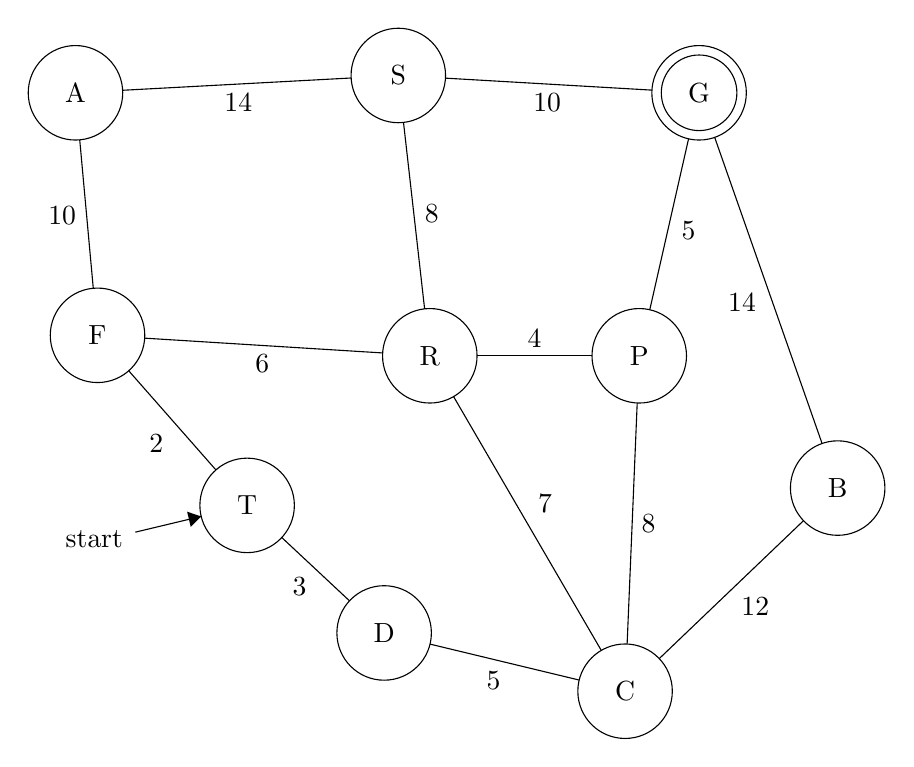
\begin{tikzpicture}[scale=0.2]
    \tikzstyle{every node}+=[inner sep=0pt]
    \draw (36.6,-29.3) circle (3) node {R};
    \draw (15.5,-28) circle (3) node {F};
    \draw (49.9,-29.3) circle (3) node {P};
    \draw (34.6,-11.5) circle (3) node {S};
    \draw (33.7,-46.9) circle (3) node {D};
    \draw (14.1,-12.6) circle (3) node {A};
    \draw (25,-38.8) circle (3) node {T};
    \draw (53.7,-12.6) circle (3) node {G};
    \draw (53.7,-12.6) circle (2.4);
    \draw (49,-50.6) circle (3) node {C};
    \draw (62.5,-37.7) circle (3) node {B};
    \draw (46.9,-29.3) -- (39.6,-29.3);
    \draw (43.25,-28.8) node[above] {4};
    \draw (14.37,-15.59) -- (15.23,-25.01);
    \draw (14.17,-20.37) node[left] {10};
    \draw (17.1,-12.44) -- (31.6,-11.66);
    \draw (24.44,-12.63) node[below] {14};
    \draw (17.48,-30.25) -- (23.02,-36.55);
    \draw (19.71,-34.85) node[left] {2};
    \draw (36.62,-47.61) -- (46.08,-49.89);
    \draw (40.65,-49.32) node[below] {5};
    \draw (47.49,-48.01) -- (38.11,-31.89);
    \draw (43.45,-38.71) node[right] {7};
    \draw (37.6,-11.67) -- (50.7,-12.43);
    \draw (44.05,-12.63) node[below] {10};
    \draw (54.69,-15.43) -- (61.51,-34.87);
    \draw (57.34,-25.9) node[left] {14};
    \draw (36.27,-26.32) -- (34.93,-14.48);
    \draw (36.26,-20.29) node[right] {8};
    \draw (49.13,-47.6) -- (49.77,-32.3);
    \draw (50.01,-39.97) node[right] {8};
    \draw (18.49,-28.18) -- (33.61,-29.12);
    \draw (25.97,-29.21) node[below] {6};
    \draw (50.57,-26.37) -- (53.03,-15.53);
    \draw (52.55,-21.34) node[right] {5};
    \draw (51.17,-48.53) -- (60.33,-39.77);
    \draw (57.27,-44.63) node[below] {12};
    \draw (27.2,-40.84) -- (31.5,-44.86);
    \draw (28.33,-43.33) node[below] {3};
    \draw (17.9,-40.5) -- (22.08,-39.5);
    \draw (17.14,-40.93) node[left] {start};
    \fill (22.08,-39.5) -- (21.19,-39.2) -- (21.42,-40.17);
  \end{tikzpicture}
\end{center}
\clearpage

\begin{enumerate}[(a)]
  \item Greedy Best First Search
  \begin{center}
    \begin{tabular}{|c|c|p{6cm}|c|}
      \hline
      Path & Current Node & Neighbors & Choice \\ \hline
      \( \emptyset \) & T &
        D; \( f(D) = h(D) = 13 \) \newline
        F; \( f(F) = h(F) = 25 \)
        & D \\ \hline
      T & D &
        T; \( f(T) = h(T) = 22 \) \newline
        C; \( f(C) = h(C) = 12 \)
        & C \\ \hline
      T,D & C &
        D; \( f(D) = h(D) = 13 \) \newline
        R; \( f(R) = h(R) = 10 \) \newline
        P; \( f(P) = h(P) = 4 \) \newline
        B; \( f(B) = h(B) = 10 \)
        & P \\ \hline
      T,D,C & P &
        C; \( f(C) = h(C) = 12 \) \newline
        R; \( f(R) = h(R) = 10 \) \newline
        G; \( f(G) = h(G) = 0 \)
        & G \\ \hline
    \end{tabular}
  \end{center}
  Path: T,D,C,P,G
  \item A* Search
  \begin{center}
    \begin{tabular}{|c|c|p{8cm}|c|}
      \hline
      Path & Current Node & Neighbors & Choice \\ \hline
      \( \emptyset \) & T &
        D; \( g(D) = 3; h(D) = 13; f(D) = 16 \) \newline
        F; \( g(F) = 2; h(F) = 25; f(F) = 27 \)
        & D \\ \hline
      T & D &
        T; \( g(T) = 6; h(T) = 22; f(T) = 28 \) \newline
        C; \( g(C) = 8; h(C) = 12; f(C) = 20 \)
        & C \\ \hline
      T,D & C &
        D; \( g(D) = 13; h(D) = 13; f(D) = 26 \) \newline
        R; \( g(R) = 15; h(R) = 10; f(R) = 25 \) \newline
        P; \( g(P) = 16; h(P) = 4; f(P) = 20 \) \newline
        B; \( g(B) = 20; h(B) = 10; f(B) = 30 \)
        & P \\ \hline
      T,C,D & P &
        C; \( g(C) = 24; h(C) = 12; f(C) = 36 \) \newline
        R; \( g(R) = 20; h(R) = 10; f(R) = 30 \) \newline
        G; \( g(G) = 21; h(G) = 0; f(G) = 21 \)
        & G \\ \hline
    \end{tabular}
  \end{center}
  Path: T,D,C,P,G
  \item The optimal solution is the path T,F,R,P,G. A* returns a suboptimal
  path because it factors \( h(n) \) too heavily into the heuristic, and
  \( h(n) \) overestimates the cost for some nodes. This is evident since
  \( h(F) > h(D) \) which causes \( f(F) > f(D) \) even though F is the node
  that has the lowest cost to get to the goal.
\end{enumerate}

\subsection*{Problem 2}
Describe Hill-climbing search. What are some of its limitations?
\par Hill-climbing search would traverse the nodes and choose a path according
to whichever got it closer to the goal (by some heuristic). If the path to the
goal requires taking a node that the heuristic considers to be further away,
the hill-climbing algorithm would get stuck and never even consider that path.

\subsection*{Problem 3}
Look at \textit{Figure} 5.4 on Page 166 of the R\&N book. Fill in the following
\textbf{3 player} minimax search tree.
\begin{center}
  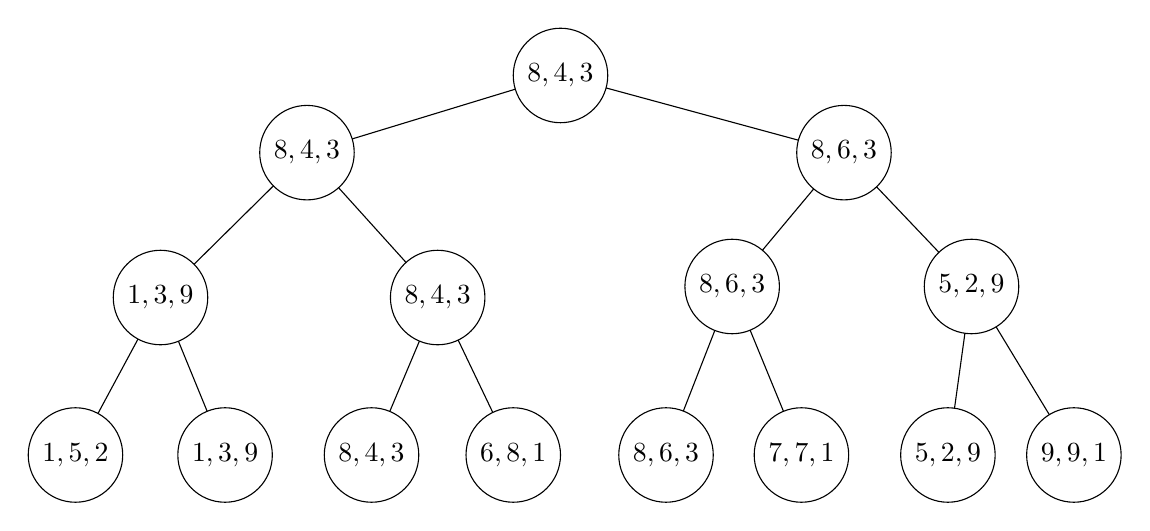
\begin{tikzpicture}[scale=0.2]
    \tikzstyle{every node}+=[inner sep=0pt]
    \draw (13.1,-20.2) circle (3) node {\( 1,3,9 \)};
    \draw (30.7,-20.2) circle (3) node {\( 8,4,3 \)};
    \draw (17.2,-30.2) circle (3) node {\( 1,3,9 \)};
    \draw (22.4,-11) circle (3) node {\( 8,4,3 \)};
    \draw (7.7,-30.2) circle (3) node {\( 1,5,2 \)};
    \draw (26.5,-30.2) circle (3) node {\( 8,4,3 \)};
    \draw (38.5,-6.1) circle (3) node {\( 8,4,3 \)};
    \draw (35.5,-30.2) circle (3) node {\( 6,8,1 \)};
    \draw (56.5,-11) circle (3) node {\( 8,6,3 \)};
    \draw (49.4,-19.5) circle (3) node {\( 8,6,3 \)};
    \draw (64.6,-19.5) circle (3) node {\( 5,2,9 \)};
    \draw (45.2,-30.2) circle (3) node {\( 8,6,3 \)};
    \draw (53.8,-30.2) circle (3) node {\( 7,7,1 \)};
    \draw (63.1,-30.2) circle (3) node {\( 5,2,9 \)};
    \draw (71.1,-30.2) circle (3) node {\( 9,9,1 \)};
    \draw (20.27,-13.11) -- (15.23,-18.09);
    \draw (24.41,-13.23) -- (28.69,-17.97);
    \draw (11.67,-22.84) -- (9.13,-27.56);
    \draw (29.54,-22.97) -- (27.66,-27.43);
    \draw (14.24,-22.98) -- (16.06,-27.42);
    \draw (32,-22.9) -- (34.2,-27.5);
    \draw (41.39,-6.89) -- (53.61,-10.21);
    \draw (54.58,-13.3) -- (51.32,-17.2);
    \draw (58.57,-13.17) -- (62.53,-17.33);
    \draw (35.63,-6.97) -- (25.27,-10.13);
    \draw (48.3,-22.29) -- (46.3,-27.41);
    \draw (50.54,-22.27) -- (52.66,-27.43);
    \draw (64.18,-22.47) -- (63.52,-27.23);
    \draw (66.16,-22.06) -- (69.54,-27.64);
  \end{tikzpicture}
\end{center}

\subsection*{Problem 4}
Create and fill-in a Minimax search tree for a 9 token game of Nim. Assume
that MAX makes the first move. Fill in the utility value for each node
generated. \\
Nodes colored blue have a utility of 1 and can lead to MIN's victory if played
right.
\begin{center}
  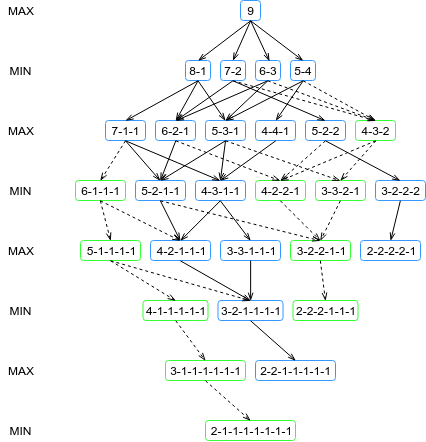
\includegraphics[width=14cm]{assets/hw_03_04.png}
\end{center}

\begin{center}
  If you have any questions, comments, or concerns, please contact me at
  alvin@omgimanerd.tech
\end{center}

\end{document}
